\section{The payoff curve}\label{sec:payoff}

Every result in the paper rests on the shape of $v$. The next theorem shows
that it is single peaked for every learning and detection technology that
satisfies \cref{ass:Q,ass:phi,ass:credit}.

\begin{assumption}[Interior reading and learning potential]\label{ass:interior}
(a) Reading the first paper is worth its time: $b\,[\partial_R\ln Q(0,P)+\theta\Delta\varphi'(0)]>1$ for all $P>0$.
(b) A thin literature is worth reading: for some $\varrho>0$,
\[
\nu_0(\varrho)\equiv\lim_{P\downarrow 0}\frac{Q(\varrho P,P)-1}{P}-\frac{\varrho}{b}-\theta\big[\lambda-\Delta\varphi(\varrho)\big]-\theta_c\lambda_c>0.
\]
\end{assumption}

Part (b) compares, at the first papers of a topic, the gain from learning along
the ray $R=\varrho P$ with the time spent reading and the overlap risk. In the
example it reads $\sup_\varrho\{\gamma\beta\varrho/(1+\varrho)-\varrho/b-\theta[\lambda-\Delta(1-e^{-\sigma\varrho})]\}>\theta_c\lambda_c$.

\begin{theorem}[The payoff curve]\label{thm:v}
Under \cref{ass:Q,ass:phi,ass:credit}:
\begin{enumerate}[label=(\roman*)]
\item $v$ is continuous on $\R_+$, $v(0)=1$, $v(P)\ge e^{-(\theta\lambda+\theta_c\lambda_c)P}>0$ and $\lim_{P\to\infty}v(P)=0$.
\item $\ln v$ is concave on $(0,\infty)$. Under \cref{ass:interior}(a) it is strictly concave.
\item Under \cref{ass:interior}, there is a unique $\Phat\in(0,\infty)$ such that $v$ is strictly increasing on $[0,\Phat]$ and strictly decreasing on $[\Phat,\infty)$, with $\vhat\equiv v(\Phat)>1$. For every $F\in(0,\vhat)$ the equation $v(P)=F$ has exactly one root above $\Phat$.
\item (Envelope) $v$ is differentiable on $(0,\infty)$ with
\begin{equation}\label{eq:envelope}
\frac{v'(P)}{v(P)}=\underbrace{\partial_P\ln Q(R^*,P)}_{\text{more to learn from}}\;-\;\underbrace{\theta\big[\lambda-\Delta\big(\varphi(c^*)-c^*\varphi'(c^*)\big)\big]-\theta_c\lambda_c}_{\text{more to miss}},
\end{equation}
where $R^*=b\,r^*(P)$ and $c^*=R^*/P$.
\item The optimal reading share $r^*(P)$ is unique and nondecreasing in $P$. Papers per researcher, $a\,x^*(P)$, are nonincreasing in density.
\end{enumerate}
\end{theorem}

The proof (\cref{app:proofs}) rests on one observation. $\ln g$ is
\emph{jointly} concave in reading time and density. $\ln(1-r)$ and $\ln Q$ are
concave by assumption. The erosion exponent
$-\theta\lambda P+\theta\Delta\,P\varphi(R/P)-\theta_c\lambda_cP$ is linear plus
the perspective of the concave function $\varphi$, and perspectives preserve
concavity. Maximising a jointly concave function over one argument leaves a
concave function of the other, so $\ln v$ is concave. A log-concave function
that starts at one, rises, and vanishes at infinity is single peaked. Part (v)
follows from Topkis's theorem: $\partial^2\ln C/\partial R\,\partial
P=-\theta\Delta\varphi''(c)\,c/P\ge 0$ and $\ln Q$ is supermodular, so reading
and density are complements.

The theorem needs no parametric assumption, and its conditions are economic:
no increasing returns to reading, and diminishing returns to search. Note what
it does \emph{not} need. Duplicates may keep most of their credit, since only
$\lambda>\ell$ is required. The single peak comes from overlap that goes
unread, not from an assumption that overlap is worthless.

\begin{remark}[Where the hump comes from, and what the theorem rules out]\label{rem:scope}
The fall in $v$ comes from \emph{bounded absorption}. What a researcher can
learn is bounded in density ($\bar Q(R)<\infty$) and what she can read is
bounded by $b$, while the expected number of covering papers, $\theta P$,
grows linearly with the literature. Any model with these two features has a
falling payoff at high density. Joint concavity of $\ln Q$ is what makes the
rise and the fall meet at a single peak. It rules out complementarities among
the papers one reads, for example a literature that becomes useful only once a
critical mass of results can be combined. With such complementarities $\ln v$
can have several local peaks, topics can have more than one stable size, and
the comparative statics below apply locally around each falling-side crossing.
We keep the concave case. It is the natural benchmark, and the arXiv returns
profile (Fact~\ref{fact:hump}) shows a single hump.
\end{remark}

\begin{figure}[t]
\centering
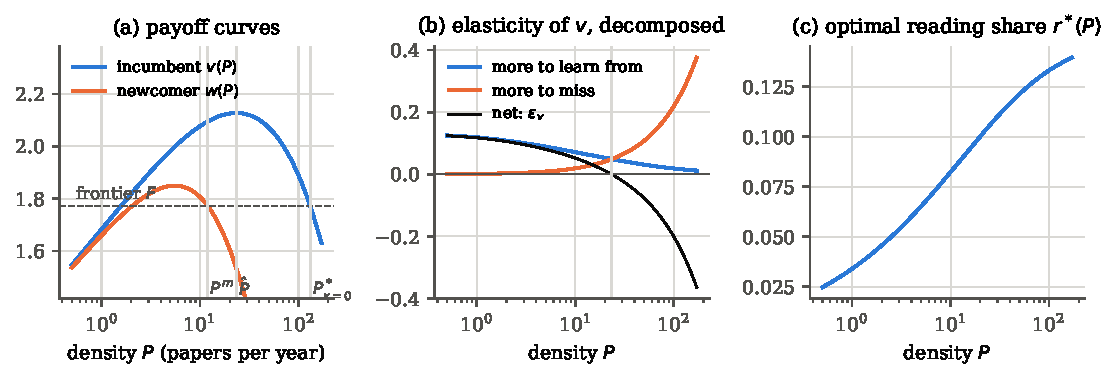
\includegraphics[width=\textwidth]{figures/fig1_payoff_curve.pdf}
\caption{The payoff curve and its two forces. Left: $v(P)$ and the newcomer's
payoff $w(P)=v(P)(1-P/b_c)^\nu$ in the calibrated model, with the peak $\Phat$,
the mature density $P^m$ where $w=F$, and the speed limit $b_c$ at which $w$
vanishes. Right: the decomposition \eqref{eq:envelope} of $v'/v$ into the
learning and overlap terms, and the optimal reading share.}
\label{fig:payoff}
\end{figure}

\paragraph{The value of time.} The envelope theorem also prices every speed-up
inside a topic.

\begin{lemma}[Time shares]\label{lem:timeshares}
At a fixed density, $\partial\ln v/\partial\ln b=r^*(P)/(1-r^*(P))$, while a
faster production speed raises a researcher's payoff by $\dd\ln a$. A speed-up
of a task that takes a share $s_k$ of her time ($s_r=r^*$ for reading,
$s_x=x^*$ for production) by $\dd\ln(\text{speed})$ saves $s_k\,\dd\ln(\text{speed})$
of her time and raises her payoff by $s_k\,\dd\ln(\text{speed})/x^*(P)$. Per unit
of time saved, every speed-up is worth the same, $1/x^*(P)$.
\end{lemma}

The proof is two lines (\cref{app:proofs}). By the envelope theorem
$\partial\ln v/\partial\ln b=r\,\partial_R\ln(QC)\,b$, and the first-order
condition sets $b\,\partial_R\ln(QC)=1/(1-r)$. A 30\% faster reader in a topic
where reading takes 7\% of time therefore gains about two log points, and a
30\% faster producer about 26. The difference is the share of time each task
takes, not anything about entry. It is entry that ranks tools whose value per
hour saved is the same, and \cref{sec:ai} shows how.

\paragraph{The sign of the spillover.} Let one more paper appear in a topic. By
the envelope theorem, the change in every other member's payoff is exactly
$a\,v'(P)$. The researchers' own reallocation of time is second order.

\begin{proposition}[Spillover sign]\label{prop:externality}
An additional paper in a topic of density $P$ changes the per-period payoff of
each incumbent by $a\,v'(P)$. The change is positive for $P<\Phat$ (more to
learn from) and negative for $P>\Phat$ (more to miss).
\end{proposition}

The sign of the spillover is therefore \emph{derived}, not assumed. A paper
helps its topic when the topic is thin and hurts it when the topic is dense.
Overproduction is not built in. Whether science is overcrowded depends on
where equilibrium places topics on $v$. That is the subject of the next two
sections.
